This chapter introduces a new proof-of-concept framework called \textit{ILP(RL)}, a new learning framework for solving MDP problems using inductive learning with ILASP and planning with ASP.
The development of this framework is one of the main objectives of this project and we explain the framework in details in this Chapter.

\section{Overview}
\label{sec:overview}

\begin{figure}[!htb]
\centering
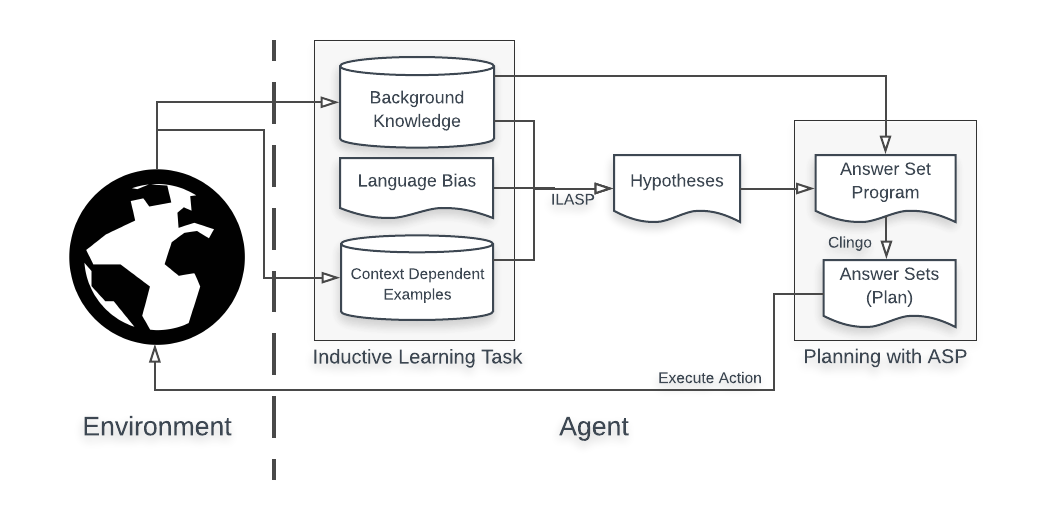
\includegraphics[width=1.0\textwidth]{./figures/architecture}
\caption{ILP(RL) overview}
\label{fig:ILPRL_overview}
\end{figure}

\begin{algorithm}
\caption{ILP(RL) Algorithm}
\begin{algorithmic}[1]
\label{algo:ILPRL}
\renewcommand{\algorithmicrequire}{\textbf{Input:}}
\State \textbf{Input:}
\State \ \ \ \ \ \ States $S = \{ 1, ..., n\textsubscript{x}\}$
\State \ \ \ \ \ \ Actions $A = \{ 1, ..., n\textsubscript{a}\} A: X \rightarrow A$
\State \ \ \ \ \ \ States transition $T: X \times A \rightarrow X$
\State \ \ \ \ \ \ $\epsilon \in [0,1]$
\State \ \ \ \ \ \ Background knowledge for ILASP and ASP $B$
\State \ \ \ \ \ \ Language bias $S\textsubscript{M}$ \\

\Procedure{ILP(RL)}{S, A, T, $\epsilon$, B, S\textsubscript{M}}
\State $H = \emptyset$
\State $E = \emptyset$
\State Start s $\in$ S
\While s is not terminal 
\State $a \leftarrow POLICY(B, H, s, A, \epsilon)$ \\
\space
\LineComment{observe the next state $s^\prime$ by taking action a}
\State $s^\prime \leftarrow T(s,a)$
\space
\LineComment{generate a positive example}
\State $e \leftarrow MakeDCPI(s^\prime, s, a) $ 
\State $E = E + e$
\space
\LineComment{if the current B $\cup$ H without language bias does not cover E, update H}
\If {$ ILASP(B \cup H, S\textsubscript{M}=\emptyset, E) == UNSATISFIABLE$}
\State $H = ILASP(B, S\textsubscript{M}, E)$
\EndIf
\State $Update(B)$
\EndWhile
\EndProcedure
\end{algorithmic}
\end{algorithm}

The overall architecture of ILP(RL), is shown in Figure \ref{fig:ILPRL_overview}. 
ILP(RL) mainly consists of two components: inductive learning with ILASP and planning with ASP. 

The first step is inductive learning. An agent interacts with an unknown environment, 
and receives state transition experiences as context dependent examples. 
Together with pre-defined background knowledge and language bias, these examples are used to inductively learn and improve hypotheses, which are state transition function in the environment.

The second step is ASP planning. The interaction with the environment also gives the agent information about the environment, such as locations of walls or a terminal state. 
The agent remembers these information as background knowledge, and, 
together with the learnt hypotheses, uses them to make an action plan by solving an ASP program.
The plan is a sequence of actions and it navigates the agent in the environment.

The agent iteratively executes this cycle in order to learn and improve the hypotheses as well as an action planning. 
Mechanisms of each step are explained in details in the following sections.

\section{Environment}
\label{sec:environment}
Since there is no existing base frameworks for ILP(RL), our focus on this project is to develop a preliminary version of the framework. 
Therefore, we use a very simple environment that allows us to see the potentials of our proposed architecture.
The base environment is a simple grid maze, and we assume that the environment is a discrete deterministic environment. 

We use a simple example to explain the environment as shown in Figure \ref{environment_example}.
States are expressed as X and Y coordinates. In Figure \ref{environment_example}, for example, the agent is located at \{X=2, Y=4\}.
The agent can take one of four possible actions at each time: up, down right and left.
Every time the agent takes an action, the agent receives the following experiences: a reward R\textsubscript{t}, the next state S\textsubscript{t+1} and surrounding information of the current state.
The base environment mainly consists of three different elements: a goal, walls and paths.
The goal cell is the terminal state and the agent receives a positive reward when the agent receives a negative reward in any states except the terminal state.
When the agent reaches the terminal state, the agent receives a positive reward and the current episode is complete. 
Since the agent's goal is to maximise the total estimate rewards over time, this goal is equivalent to finding the shortest path from a starting state to a terminal state.

We also assume that, unlike an agent with other RL algorithms, the agent can see states of vertical and horizontal, but not diagonal, states around the agent. 
This assumption allows a agent to learn a state transition in the environment using inductive learning. For example, the agent at \{X=2, Y=4\} can see that there are walls at \{X=1, Y=4\} and \{X=2, Y=5\}.
More details of how to use these surrounding information is described in \ref{sec:inductive_learning_task}.

The applicability for a more complex environment is not considered in this project and it is discussed in Further Research in Section \ref{sec:further_research}.

% The environment is provided outside of our algorithm,
\begin{figure}[!htb]
\centering
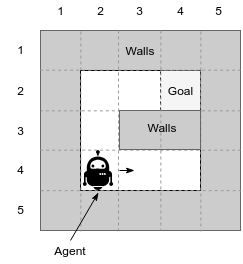
\includegraphics[width=0.4\textwidth]{./figures/environment_example}
\caption{5$\times$5 grid maze example}
\label{environment_example}
\end{figure}

\section{Inductive Learning Task}
\label{sec:inductive_learning_task}
The first step is to construct a learning task using ILASP. The objective of the inductive learning is to learn state transitions in a given environment, which is used for generating an action plan at later steps.
The target hypotheses are specified as follows:

\begin{equation}
\begin{split}
&\textsf{state\_after(V1):-adjacent(right, V0, V1), state\_before(V1), action(right), wall(V0).}\\
&\textsf{state\_after(V0):-adjacent(right, V0, V1), state\_before(V1), action(right), not wall(V0).}\\
&\textsf{state\_after(V1):-adjacent(left, V0, V1), state\_before(V1), action(left), wall(V0).}\\
&\textsf{state\_after(V0):-adjacent(left, V0, V1), state\_before(V1), action(left), not wall(V0).}\\
&\textsf{state\_after(V1):-adjacent(down, V0, V1), state\_before(V1), action(down), wall(V0).}\\
&\textsf{state\_after(V0):-adjacent(down, V0, V1), state\_before(V1), action(down), not wall(V0).}\\
&\textsf{state\_after(V1):-adjacent(up, V0, V1), state\_before(V1),  action(up), wall(V0).}\\
&\textsf{state\_after(V0):-adjacent(up, V0, V1), state\_before(V1), action(up), not wall(V0).}
\end{split}
\label{target_hypothesis}
\end{equation}

where \textsf{state\_after} is the next state S\textsubscript{t+1}, \textsf{state\_before} is the current state S\textsubscript{t}. \textsf{action} is an action A\textsubscript{t} taken by the agent.
\textsf{adjacent(D, V0, V1)} specifies that V0 is next to V1 in the direction of D. For example, \textsf{adjacent(right, V0, V1)} means V0 is right next to V1. 
\textsf{wall(V)} and \textsf{not wall(V)} specify whether a state is a wall or not wall in a state V respectively.
We describe the details of how to construct the background knowledge, context dependent examples and the language bias in the following sections, and these are the necessary components for the agent to learn the target hypotheses.
The summary of a full ILASP learning task can be found in Appendix \ref{chap:learning_tasks}.
% Similar to other RL algorithms, an agent explores an environment by taking actions, which generates experiences. 
% These experiences need to be translated into ASP syntax and 
% and are recorded in as context dependent examples. 
% a positive example and background knowledge.
% Positive examples and background knowledge are used by ILASP for inductive learning, and background knowledge is used by both ILASP and ASP for solving for answer sets.

\subsection{Background Knowledge}
\label{subsec:background_knowledge}
First we define necessary background knowledge for the inductive learning.
In order to learn the state transition for each direction as shown in \ref{target_hypothesis}, we need to define the meaning of "being next to" a state.
This is defined as a rule \textit{adjacent}, which is of the form:

\begin{equation} \label{eq:adjacent}
\begin{split}
&\textsf{adjacent(right, (X+1,Y),(X,Y)):-cell((X,Y)), cell((X+1,Y)).} \\
&\textsf{adjacent(left,(X,Y),  (X+1,Y)):-cell((X,Y)), cell((X+1,Y)).} \\
&\textsf{adjacent(down, (X,Y+1),(X,Y)):-cell((X,Y)), cell((X,Y+1)).} \\
&\textsf{adjacent(up,   (X,Y),  (X,Y+1)):-cell((X,Y)), cell((X,Y+1)).} \\
\end{split}
\end{equation}

where \textsf{cell} corresponds to a state, and \textsf{X} and \textsf{Y} represent x-coordinate and y-coordinate respectively.
The rules \ref{eq:adjacent} are given as background knowledge and allow the agent to understand the relation of two adjacent states.
\textit{cell((X,Y))} is defined as follows:
\begin{equation} \label{eq:cell}
\begin{split}
    &\textsf{cell((0..X, 0..Y)).}
\end{split}
\end{equation}

where, \textsf{X} and \textsf{Y} are the size of width and height of an environment respectively. 
For example, a grid maze shown in Figure\ref{environment_example} has a height and width of 4, thus the type cell is defined in the background knowledge as \textsf{cell((0..4, 0..4))}.

\subsection{Context Dependent Examples}
Context dependent examples contain actual state transition that the agent gains by interacting with an environment. Since all the interactions with the environment are examples of valid moves,
they are used as positive examples. A positive example is expressed as a following ASP form:
\begin{equation}
\begin{split}
    \textsf{\#pos}(\{E\SPSB{inc}{ILP(RL)}\}, \{E\SPSB{exc}{ILP(RL)}\}, \{C\textsubscript{ILP(RL)}\})
\end{split}
\end{equation}

It is equivalent to context-dependent partial interpretation (CDPI) in  $ILP_{LAS}^{context}$. 
As defined in the Equation \ref{eq:cdpi}, CDPI is of the form $\langle e, C \rangle$ where $e = \langle E\textsuperscript{inc}, E\textsuperscript{exc} \rangle$. 
Each of the component in CDPI in ILP(RL) is defined as follows:

\begin{defn}\label{def:ILPRL_context}
$C\textsubscript{ILP(RL)}$ contains an action a\textsubscript{t}, the current state $s\textsubscript{t}$, and adjacent walls of $s\textsubscript{t}$.
\label{def:context}
\end{defn}

\begin{defn} \label{def:ILPRL_inc}
$E\SPSB{inc}{ILP(RL)}$ includes $s\textsubscript{t+1} \in S$ such that:
\begin{itemize}
\item s\textsubscript{t+1} = s\textsuperscript{*}\textsubscript{t+1}
\item $ \forall A \in AS(B \cup H\textsubscript{t} \cup C\textsubscript{ILP(RL)})|$ s\textsubscript{t+1} $\not\in A$
\end{itemize}
\end{defn}

\begin{defn} \label{def:ILPRL_exc}
$E\SPSB{exc}{ILP(RL)}$ includes $s\textsubscript{t+1} \in S$ such that:
\begin{itemize}
\item $s\textsubscript{t+1} \neq s\textsuperscript{*}\textsubscript{t+1}$
\item $ \exists A \in AS(B \cup H\textsubscript{t} \cup C\textsubscript{ILP(RL)})|$ s\textsubscript{t+1} $\in A$
\end{itemize}
\end{defn}

where $s\textsuperscript{*}\textsubscript{t+1}$ is the true next state where the agent is at $t+1$, 
$B$ is the background knowledge, $H\textsubscript{t}$ is the hypotheses at $t$, $S$ is all the states in the environment.

% For context C, a\textsubscript{t} is translated int \textit{action((a))}, s\textsubscript{t} is translated into \textit{state\_before((x,y))}, and adjacent walls of s\textsubscript{t} are translated into \textit{wall((x$^\prime$,y$^\prime$))}.

% In this report, we assume that part of context contains only whether a wall exists or not, with the presence of a wall, the agent cannot move to the state where a wall exists.

% \subsubsection{Positive examples in ASP syntax}
% \label{subsubsec:positive_examples_asp_syntax}

% For example, if the agent takes an action "up" to move from (1,1) to (1,2), all other states that the agent could have taken but did not are exclusions ((1,0), (1,1), (0,1) and (2,1) in this case).
% context examples include state\_before((X1,Y1)), which represents the position of the agent in x and y axis before an action is taken,
% action(A) is the action the agent has taken, and surrounding information, such as surrounding walls.

% Rewards are not used.
% (Discussed in details in Chapter XX).

% \textcolor{red}{There is no negative example as XXXX.}
% Using these positive examples, the agent is able to learn and improve hypothesis as it explore the environment and encounters new scenarios.
\begin{examp} \normalfont (Context dependent examples).

\begin{figure}[!htb]
\centering
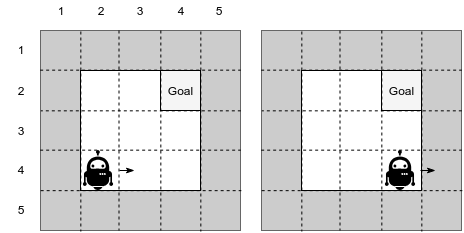
\includegraphics[width=0.8\textwidth]{./figures/pipeline_example1}
\caption{5$\times$5 grid maze example (context dependent example)}
\label{example_pos_example}
\end{figure}

We use a simple $5 \times 5$ grid maze environment to highlight how an agent gains a positive example.
Suppose $H\textsubscript{t}=\emptyset$ and an agent takes an action "right" to move from $(1,3)$ to $(2,3)$ cell, as shown on the left in Figure \ref{example_pos_example}.
$a\textsubscript{t}$ is "right", $s\textsubscript{t}$ is $(1,3)$ and $s^*\textsubscript{t}$ is $(2,3)$.
According to the Definition \ref{def:ILPRL_inc}, $A=\emptyset$ since $H\textsubscript{t}=\emptyset$, thus \textsf{state\_after((2,3))} is in $E\SPSB{exc}{ILP(RL)}$, $A=\emptyset$ is there is no exclusions in this case.
$C\textsubscript{ILP(RL)}$ includes $a\textsubscript{t}$, $s\textsubscript{t}$ and adjacent walls of $s\textsubscript{t}$.
The following positive example is generated.

\begin{equation}
\begin{split}
    \textsf{\#pos(} & \textsf{\{state\_after((2,3))\},}\\
                    & \textsf{\{\},} \\
    & \textsf{\{state\_before((1,3)). action(right). wall((0, 3)). wall((1, 4)).\})}
\end{split}
\end{equation}

The next example illustrates a case when the agent tries to move to a state where a wall is. As shown on the right in Figure \ref{example_pos_example}, the agent is at $(3,3)$ and tries to move to a state $(3,4)$ by taking an action "right", as shown on the left in Figure \ref{example_pos_example}. 
In this case, however, there is a wall at $(4,3)$ and therefore the agent cannot go to that state. Because of the blocking wall, $s\textsubscript{t} = s^*\textsubscript{t+1} = (4,4)$.
The same the previous case, suppose $H = \emptyset$ and therefore $A = \emptyset$.
% All other alternative next adjacent states S\textsubscript{t+1} (4,3), (3,4), (5,4) and (4,5) are exclusions, and the contexts are collected.
From this example, the following positive example is generated:
\textcolor{red}{TODO UPDATE this example}
\begin{equation}
\begin{split}
\textsf{\#pos(} & \textsf{\{state\_after((4,4))\}}, \\
                & \textsf{\{state\_after((4,3)),state\_after((3,4)),state\_after((5,4)),state\_after((4,5))\}} \\
                & \textsf{\{state\_before((4,4)). action(right). wall((5,4)). wall((4,5)).\}).}
\end{split}
\end{equation}

\end{examp}
\label{state_transition_example}

\subsection{Language Bias}
\label{subsec:language_bias}
We now define a search space using a language bias specified by \textit{mode declaration}.
As defined in \ref{def:las_context}, $H \subseteq S\textsubscript{M}$ for $ILP_{LAS}^{context}$, thus in order to learn the target hypotheses, $S\textsubscript{M}$ is specified as follows:
\begin{equation} \label{eq:sm}
\begin{split}
&\textsf{\#modeh(state\_after(var(cell))).}\\
&\textsf{\#modeb(1, adjacent(const(action), var(cell), var(cell)), (positive)).} \\
&\textsf{\#modeb(1, state\_before(var(cell)), (positive)).} \\
&\textsf{\#modeb(1, action(const(action)),(positive)).} \\
&\textsf{\#modeb(1, wall(var(cell))).} \\
\end{split}
\end{equation}

where \textsf{\#modeh} and \textsf{\#modeb} are the \textit{normal head declarations} and the \textit{body declarations}. 
The first argument of each \textsf{\#modeb} specifies the maximum number of times that \textsf{\#modeb} can be used in each rule (also called \textit{recall}) \cite{Law2017}, 
which we specify $1$ for \textsf{\#modeb} in ILP(RL). \textsf{var(t)} is a placeholder for a variable of \textit{type} \textsf{t}. In \ref{eq:sm}, we use \textsf{cell} for the variable type, which is grounded using \textsf{cell} specified in \ref{eq:cell} in the background knowledge.
\textsf{const(t)} is a placeholder for a constant term of type \textsf{t}, and type \textsf{t} must be specified as \textsf{\#constant(t, c)}, where \textsf{c} is a constant term., 
\textsf{const(t)} is specified as follows:

\begin{equation}
\begin{split}
&\textsf{\#constant(action, right).}\\
&\textsf{\#constant(action, left).}\\
&\textsf{\#constant(action, down).}\\
&\textsf{\#constant(action, up).}
\end{split}
\end{equation}

\textsf{action} type is specified as a constant since ILP(RL) needs to learn a different hypothesis of state transitions for each direction based on the context dependent examples that the agent collects..

\textsf{(positive)} in \textsf{\#modeb} specifies that the body predicates only appear as positive and not negation as failure, which reduces the search space. We use \textsf{(positive)} for all \textsf{\#modeb} except \textsf{wall}. Thus \textsf{wall(var(cell))} could appear as \textsf{not wall} in a hypothesis, and all other body predicates should only be positive.

Finally, we define \textsf{\#max\_penalty} to specify the maximum size of the hypothesis. By default it is 15, however our target hypotheses defined in \ref{target_hypothesis} is larger than 15, and thus it is increased to 50.
Increasing \#max\_penalty allows ILASP to learn longer hypotheses at the expense of longer computation.

\subsection{Hypothesis}
\label{sebsec:hypothesis}
Having defined the $ILP_{LAS}^{context}$ task $T = \langle B, S\textsubscript{M}, E\textsuperscript{+}, E\textsuperscript{-} \rangle$, ILP(RL) is able to learn hypotheses $H$. 
Since $B$ and $S\textsubscript{M}$ are fixed, the hypotheses vary based on context dependent examples that the agent accumulates by interacting with an environment.
For example, in the early phase of learning, the agent does not have many positive examples, and learns a hypothesis that is subset of the full target hypotheses that the agent could learn in the environment. Thus ILP(RL) needs to iteratively improves the hypotheses as illustrated in Figure \ref{fig:ILPRL_overview}.
As specified in line 19 of Algorithm \label{algo:ILPRL}, $ILP_{LAS}^{context}$ is executed when the current hypotheses do not cover the new context example.
If the current hypotheses cover the new positive example, there is no need to re-execute ILASP.
% ILP(RL) runs $ILP_{LAS}^{context}$ to relearn H\textsubscript{new} if and only if $\forall$$\langle$ e, C$\rangle$ $\in$ E\textsuperscript{+}, $\exists$A $\in$ Answer Sets (B $\cup$ C $\cup$ H) such that A extends e
% \end{defn}
% where H is the current hypotheses that the agent has learnt so far. 

The learnt hypotheses will be used for ASP planning, which we describe in the next section.

\begin{examp} \normalfont (Hypothesis).
Using the context dependent examples illustrated in Example \ref{example_pos_example}, we explain how the agent learns hypotheses.
Suppose that the agent takes an action "right" and gains one positive example, as shown on the right in Example \ref{example_pos_example}. 
The full learning task for this simple case is shown as follows:

\lstinputlisting[
  caption  = {Learning task example},
]{learning_task_example1.pl}
From the above learning task, ILASP learns the following hypothesis.
\begin{equation*}
\begin{split}
\textsf{state\_after(V1) :- adjacent(left, V0, V1), state\_before(V0).}
\end{split}
\end{equation*}

After having learnt the hypothesis above, suppose the agent takes another action and gains one extra example as shown in Listing \ref{additional_example}.
\lstinputlisting[
  caption  = {Additional context dependent example},
  label = {additional_example}
]{learning_task_example2.pl}

The current hypothesis, does not cover the new positive example, ILP(RL) runs ILASP with the new positive example. The revised hypotheses are as follows:
\begin{equation*}
\begin{split}
XXX
\end{split}
\end{equation*}

ILP(RL) keeps improving the hypotheses this way until the target hypotheses are learnt.
\end{examp}

\section{Planning with Answer Set Programming}
\label{sec:planning}
The learnt hypotheses in the inductive learning phase are used to generate a sequence of action plan that the agent should follow.
In the following subsections, we explain how to create an ASP program and use the answer sets by the ASP to make an action plan in a maze environment.
\subsection{Answer Set Program}
\label{subsec:answer_set_program}
The ASP program should be constructed such that answer sets of the ASP program are a sequence of actions and states at each time step in ASP syntax. 
The answer set program for ILP(RL) is summarised in Listing \ref{list:asp_planning}:
\lstinputlisting[
  caption  = {Answer set program for ILP(RL)},
  label = {list:asp_planning}
]{asp_planning.pl}

First, we use the learnt hypotheses by $ILP_{LAS}^{context}$ as part of the ASP program.
In the inductive learning phase in ILP(RL), we only need to differentiate between s\textsubscript{t} and s\textsubscript{t+1} as \textsf{state\_before} and \textsf{state\_after} respectively.
However, for the planning with ASP, the answer sets contains a sequence of actions and states for more than two time steps. 
In order to capture the notion of time sequences, we modify the ASP syntax by 
adding time \textit{T}. Specifically, the following mapping is required between ILASP and ASP planning syntax.

\begin{table}[H]
\centering
\begin{tabular}{|l|p{5cm}|p{5cm}|}
% \begin{tabular}{|l|l|p{1.5cm}|p{7cm}|l|l|l|l|}
\hline
No & ILASP syntax & ASP planning syntax\\ \hline
1 & \textsf{state\_before(V)} & \textsf{state\_at(V1, T)}  \\ \hline
2 & \textsf{state\_after(V)} & \textsf{state\_at(V1, T+1)}  \\ \hline
3 & \textsf{(empty body)} & \textsf{time(T)}  \\ \hline
4 & \textsf{action(A)} & \textsf{action(A, T)}  \\ \hline
\end{tabular}
\caption{ASP syntax mapping between }
\label{table:extension_specification}
\end{table}
The conversion from (empty body) to \textsf{time(T)} means that the body of all the hypotheses include \textsf{time(T)} in ASP planning syntax.
\begin{examp} \normalfont (Mapping of ASP syntax between $ILP_{LAS}^{context}$ and ASP).

Suppose that an agent learnt the following hypothesis in inductive learning phase. 
\begin{equation*}
\begin{split}
&\textsf{state\_after(V0) :- adjacent(right, V0, V1), state\_before(V1), action(right), not wall(V0).}\\
\end{split}
\end{equation*}

This hypothesis is converted into the following for ASP planning.
\begin{equation*}
\begin{split}
&\textsf{state\_at(V0, T+1) :- time(T), adjacent(right, V0, V1), state\_at(V1, T), action(right, T), not wall(V0).}\\
\end{split}
\end{equation*}
The converted hypothesis can generate a sequence of actions and states to the right direction at more then two time steps.
\end{examp}

Second, we define a choice rule of actions, which is of the form:
\begin{equation}\label{eq:choice_rule}
\begin{split}
&\textsf{1\{action(down,T); action(up,T); action(right,T); action(left,T)\}1} \\
&\textsf{ :- time(T), not finished(T).}\\
\end{split}
\end{equation}

An action is given as a choice rule, and the choice rule states that an action must be one of four actions: \textsf{down}, \textsf{up}, \textsf{right}, or \textsf{left}
at each time step T, as defined in the maximum and minimum integers 1.
The choice rule specifies that one of four actions must be true unless \textsf{not finished(T)} or \textsf{time(T)} are satisfied, as defined in the body of the rule.
In RL scenarios, this means there is always action to be taken until the agent reaches a terminal state, 
When the agent reaches a terminal state, \textsf{finished(T)} is satisfied, otherwise time step T exceeds a maximum time steps allocated to the agent.

The maximum time steps are specified externally and it is of the form:

\begin{equation}
\begin{split}
&\textsf{time(T\textsubscript{t}..T\textsubscript{max})}
\end{split}
\end{equation}
where T\textsubscript{t} is the current time step and T\textsubscript{max} is the maximum time steps.
For example, if an agent is at time step 0, and can take actions up to 100 times within a episode until it finds a goal, \textsf{time} is defined as \textsf{time(0..100)}.

\textsf{finished(T)} determines whether the agent reaches the goal, which is defined in the following ASP form:

\begin{equation}\label{eq:asp_goal}
\begin{split}
&\textsf{finished(T):- goal(T2), time(T), T} \geq \textsf{T2.}\\
&\textsf{goal(T):- state\_at((X\textsubscript{goal}, Y\textsubscript{goal}), T), not finished(T-1).}\\
&\textsf{goalMet:- goal(T).}\\
&\textsf{:- not goalMet.}
\end{split}
\end{equation}

\textsf{state\_at((X\textsubscript{goal}, Y\textsubscript{goal}))} is the location of the goal, which is unknown to the agent in the beginning of the training.
The agent explores the environment until it finds the goal location.
In the other words, the agent cannot generate a plan to the goal until the goal is found. 
Once the agent reaches the goal and \textsf{finished(T)} is satisfied, 
there will not be any actions at time T+1 since the body of the action choice rule defined in \ref{eq:choice_rule} is not satisfied.

Next, facts of walls information are what the agent collects as context of context dependent examples, which is provided as follows:
\begin{equation}
\begin{split}
&\textsf{wall((X,Y))}\\
\end{split}
\end{equation}
 
For ASP planning part, these wall information is accumulated as background knowledge different from background knowledge for ILASP, and used it for solving ASP. 

Next, the starting state for the planning provided as part of ASP. It is the current location of the agent when the plan is generated.
\begin{equation}
\begin{split}
\textsf{state\_at((X\textsubscript{start}, Y\textsubscript{start}), T)}
\end{split}
\end{equation}

In addition, the definition of adjacent and cell type are also provided, which are the same as what was defined as background knowledge of $ILP_{LAS}^{context}$ (Equation \ref{eq:adjacent} and \ref{eq:cell})
adjacent.

Next, we need to incorporate a notion of rewards in each state. Instead of maximising the total rewards, which is the objectives of most RL methods, 
we use optimisation statements as follow. 
\begin{equation}
\begin{split}
&\textsf{\#minimize\{1, X, T: action(X,T)\}}.
\end{split}
\end{equation}

The use of optimisation statement is based on the assumption that the total rewards can be maximised by searching for optimal answer sets. 
While this works only subset of MDP, our preliminary research focuses on solving this particular MDP problem. 
    
Finally, we are only interested in a sequence of actions and corresponding states as the output of the ASP program. 
Clingo can selectively include the atoms of certain predicates in the output and hide unselected ones. 
This is specified as follows:
\begin{equation}
\begin{split}
&\textsf{\#show state\_at/2.} \\
&\textsf{\#show action/2.}
\end{split}
\end{equation}
This way the answer sets of the ASP program contains only \textsf{state\_at} and \textsf{action}.

\subsection{Plan Execution}
\label{subsec:plan_execution}
Having defined the ASP program, we describe how to use the answer sets generated by the ASP in order to execute the planning.
The output of an ASP program is of the form:
\begin{equation}
\begin{split}
&\textsf{state\_at((x\textsubscript{t},y\textsubscript{t}),t), action(a\textsubscript{t},t),}\\
&\textsf{state\_at((x\textsubscript{t+1},y\textsubscript{t+1}),t+1), action(a\textsubscript{t+1},t+1),}\\
&\textsf{state\_at((x\textsubscript{t+2},y\textsubscript{t+2}),t+2), action(a\textsubscript{t+2},t+2),}\\
&\cdots\\
&\textsf{state\_at(((x\textsubscript{t+n},y\textsubscript{t+n}),t+n), action(a\textsubscript{t+n},t+n),}\\
&\textsf{state\_at((x\textsubscript{goal},y\textsubscript{goal}),t+n+1).} 
\end{split}
\end{equation}

where \textit{n} is the number of time steps taken to reach the goal. 
\textit{action(A,T)} tells which action the agent should take at each time.
Given the answer set planning is correct, the agent follows the plan and reach the goal. 
The correctness of the planning is based on the correctness of the hypotheses as well as the wall surrounding information in the agent's background knowledge. 
For the correctness of the hypotheses, since the agent does not know all the information about the environment in the beginning of the learning,   
Clingo might not generate correct sequence of actions leading to the goals.
Also if the agent has not seen enough surrounding walls, the plan of actions might be blocked by a wall that the agent has not seen. 

\begin{examp} \normalfont (Answer Set Program).

\begin{figure}[!htb]
\centering
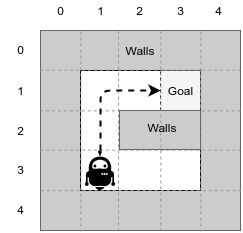
\includegraphics[width=0.4\textwidth]{./figures/asp_example}
\caption{5$\times$5 grid maze example (ASP planning)}
\label{environment_example}
\end{figure}
We use the same 5*5 grid maze as an example to highlight how the ASP planning works. 
Suppose that the agent is at (1,3) and has already found a terminal state (3,1).
Thus the agent can make an action plan to reach the goal. The ASP program for this example is provided as follows:

\lstinputlisting[
    caption  = {Answer set program for ILP(RL)},
    label = {list:asp_planning}
]{asp_planning_example.pl}

\end{examp}
    
% Together with hypothesis, the background knowledge will used to solve for answer sets program. 
% However, since hypothesis is not complete, there is more than one answer set at each time step. 
% Since one of the answer sets state\_at is correct, the rest will be in the exclusions in the answer set, 
% which is used to further improve the hypothesis in the next iteration of inductive learning.
% In this example, the following is the answer set program
% The answer set using the hypothesis XXX is 

XXX.
% The answer set using the improved hypothesis is XXX, 
% Which correctly returns a sequence of actions and predicted states.

This incorrect plan is also a source for learning a better hypothesis. 
As shown in Example XX, if the hypothesis is not a full hypotheses, outputs of ASP contain lots of \textsf{state\_at((X,Y), T)} at the same states. 
Given the agent is at one state at each time step, these duplicates are all included in exclusions, as defined in Definition \ref{def:ILPRL_exc}.

This completes the whole cycle of ILP(RL) shown in Figure \ref{fig:ILPRL_overview}.
% When the agent encounters a new environment (e.g a new wall), this new information will be added to its background, which will be used to improved the hypothesis. 
% Similarly, after executing an action by following the generated plan, the agent receives a new positive example. If the new positive example is not covered by the current hypotheses, 
% ILASP reruns using the new example to improve the hypotheses. 
% next time ILASP gets executed.
% For example,
% \begin{equation*}
% \begin{split}
% &\textsf{state\_at((1,1),1), action(right,1)}\\
% &\textsf{state\_at((2,1),2), action(right,2)}\\
% &\textsf{state\_at((3,1),3), action(right,3)}\\
% &\textsf{state\_at((4,1),4), action(right,4)}\\
% &\textsf{state\_at((5,1),5)}, \cdots
% \end{split}
% \end{equation*}
% At the start of the learning, H is usually not correct or too general, using this H will generate lots of answer sets that are not useful for the planning.
% These examples will be collected and included as exclusions of a new positive example.

\section{Exploration}
\label{exploration}
In this section, we explain exploration of ILP(RL). While the agent can learn the hypotheses and execute a planning by interacting with the environment as shown in Figure \ref{fig:ILPRL_overview},
there are mainly two reasons why ILP(RL) requires exploration. 
First, the ILP(RL) agent can only do ASP planning only if it finds a terminal state. 
Therefore the agent needs to continues exploring the environment until the terminal state is found. 
Second, even if the terminal state is known and the agent generates a planning based on the background knowledge and the hypotheses, 
this does not guarantee that the agent always finds an optimal plan.
While the agent exploit what is already learnt and follow the best plan so far,
the agent also needs to explore by taking a new action to discover a new state, which might make the agent discover an even shorter path and therefore higher total rewards in the long term.

One of the simple exploration policies in RL is called \textit{$\epsilon$-greedy policy}.
$\epsilon$-greedy policy states that an agent follows the optimal policy with probability of (1- $\epsilon$) where $\epsilon \in [0,1]$, 
and the agent takes an random action with a probability of $\epsilon$. $\epsilon$ is hyper-parameter and chosen externally.
Based on $\epsilon$-greedy policy, we define the exploration policy for ILP(RL) in \ref{alg:exploration}:
\begin{algorithm}[!htb]
\caption{ILP(RL) Exploration Policy}
\begin{algorithmic}[1]
\label{alg:exploration}
\Procedure{Policy}{}
\If {Terminal state is found}
\State
\LineComment{rand(0,1) generates a random number between 0 and 1}
\If {$rand(0,1) < \epsilon $} 
\space
\State
\LineComment{randInt(0,A) generates a uniformly random integer between 0 and $|A|$}
\State $i = randInt(0, |A|)$ 
\Return $a\textsubscript{i}$
\Else \State $a\textsubscript{i}$ = ASP Plan of ILP(RL)
\Return $a\textsubscript{i}$
\EndIf
\Else \State $i = randInt(1, |A|)$
\Return $a\textsubscript{i}$
\EndIf
\EndProcedure
\end{algorithmic}
\end{algorithm}
When the agent deviates from the planning by taking an random action and moves to a new state, the agent generates a new planning from the new state. 
Since the ILP(RL) agent does not know when the optimal plan is found, it is necessary for ILP(RL) to continues $\epsilon$-greedy strategy.

\section{Implementation}
\label{Implementation}
In this section, we describe how we developed ILP(RL) framework.
There are mainly three different components that need to be communicated: inductive learning with ILASP, planning with ASP and the external environment platform provided by VGDL with OpenAI interface.
All of them are communicated through the main driver written in Python. 
In the following section, we explain each component of ILP(RL) in details.

\subsection{Inductive Learning with ILASP}
We use ILASP2i, a inductive learning system developed in XX. 
ILASP2i is an interactive version of ILASP2, and is designed to scale with the numbers of examples. 
ILASP2i also introduces the use of context dependent examples.
The latest ILASP officially available at the time of writing is ILASP3, which is designed to work on a noisy examples. 
Our positive examples do not contain noise, state transition positive examples, and ILASP2i was sufficient for our implementation.
which is discussed in Section XX. 
Although ILASP2i is designed to work with a large number of examples, inductive learning part is the bottleneck of our framework in terms of computational time. 
We did a number of optimisation in order to mitigate this. 

The first optimisation is the frequency of running ILASP. 
As already described in Definition \ref{def:ILASP_run}, ILASP is ran only if the current hypothesis does not cover all the examples accumulated so far.
Because of this, inductive learning takes place at the very early stage of learning, which is highlighted in the experiments in Chapter XX. 

The next optimisation is through the command line. 
ILASP2i has a number of options, and we explain each option using the actual command we use to run ILASP

% \begin{minted}[]
% ILASP --version=2i FILENAME.las -ml=8 -nc --clingo5 
% \end{minted}

\begin{lstlisting}[]
    ILASP --version=2i FILENAME.las -ml=8 -nc --clingo5 
    --clingo "clingo5 --opt-strat=usc,stratify" 
    --cached-ref=PATH --max-rule-length=8
\end{lstlisting}

where,
\begin{itemize}
\item \textsf{--version=2i} specifies that we use ILASP2i.
\item \textsf{--ml=8} specified the maximum numbers of body that each rule can have. The default length is 3.
\item \textsf{--nc} means no constrains, and omits constrains from the search space. Since our target hypothesis is not a constraint, this option reduces the search space.
\item \textsf{--clingo5} generates Clingo 5 programs, which is faster, instead of Clingo 4.3.
\item \textsf{--clingo "clingo5 --opt-strat=usc,stratify"} specifies Clingo executable with the specified options. 
\textsf{usc, stratify} is unsatisfiable-core base optimisation with stratification using Gringo \cite{gringo}, a core XXX introduced in gringo version 3. REFERENCE.
\item \textsf{--cached-ref=PATH} enables the iterative mode, and keeps the output of the relevant example to a specified path, and start the learning from where it left before rather than going though all the examples.
\item \textsf{--max-rule-length=8} The default maximum number is 5.
\end{itemize}

Last optimisation is specifying search space.

Complexity. 

TODO the number of search space XX. 

\subsection{Planning with ASP}
Planning is computed using Clingo 5.

\begin{lstlisting}[]
    clingo5 --opt-strat=usc,stratify -n 0 FILENAME.lp
    --opt-mode=opt --outf=2
\end{lstlisting}

\begin{itemize}
\item \textsf{--clingo "clingo5 --opt-strat=usc,stratify"} specifies clingo executable with the specified options. 
\textsf{usc, stratify} is unsatisfiable-core base optimisation with stratification using Gringo \cite{gringo}, a core XXX introduced in gringo version 3. REFERENCE.
\item \textsf{-n 0} -n is an abbreviation of \textsf{models} to specify the maximum number of answer sets to be computed. \textsf{-n 0} means to compute all answer sets.
\item \textsf{--opt-mode=opt} computes optimal answer sets
\item \textsf{--outf=2} makes the output in JSON\footnote{http://json.org/} format
\end{itemize}

\subsection{Environment Platform}
\subsubsection{The Video Game Definition Language (VGDL)}

\begin{figure}[!ht!b]
\centering
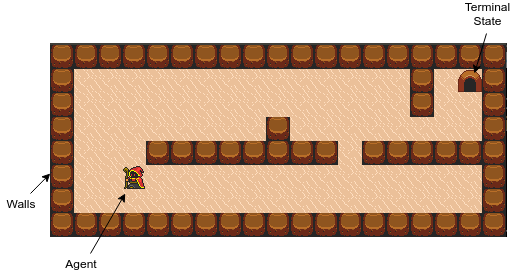
\includegraphics[width=1\textwidth]{./figures/env_sample}
\caption{Map sketch of a VGDL game (left) and it's high-level representation (right)} 
\label{VGDL_sample}
\end{figure}

We use the Video Game Definition Language (VGDL), which is a high-level description language for 2D video games providing a platform for computational intelligence research (\cite{Schaul2013}).
The VGDL allows users to easily craft their own environments, 
which makes us possible to do various experiments without relying on a default environment.

The base game we used to implement ILP(RL) is shown in Figure\ref{VGDL_sample}.
The map sketch is a plain text file and is easy to modify the configuration of the game.

\lstinputlisting[
    caption  = {VGDL description of a maze game},
    label = {list:vgdl}
]{vgdl.pl}

The behaviours of the game can be specified using VGDL as shown in \ref{list:vgdl}. 
All objects in the games can be described as a sprite in the \textit{SpriteSet}, where users can define the objects' properties.
\textit{InteractionSet} specify the effects of objects when two objects interact in the game.
\textit{TerminationSet} specify the conditions for ending the game.
The representation of each object can be specified in \textit{LevelMapping} and allows users to customise an original map.

We use PyVGDL\footnote{https://github.com/schaul/py-vgdl/}, which is a high-level VGDL on top of pygame\footnote{https://www.pygame.org}, 
a Python modules designed for writing video games.

\subsubsection{OpenAI Gym}
The VGDL platform provides an interface with OpenAI Gym (\cite{Brockman2016}), a commonly used benchmark platform for RL research.
The communication between VGDL environment and an agent, is through OpenAI Gym interface. 
\ref{list:openai} shows the functions provided by OpenAI Gym as well as the simple implementation for RL. 

In this report, an agent receives a reward of -1 for any state except the terminal state, and receives reward of +10 for the terminal state, or the goal.

% In all experiments, the agent receives -1 in any states except the goal state, where it gains a reward of 10.
% Once the agent reaches the goal, or termination state, that episode is finished and the agent start the next episode from the starting point.

\lstinputlisting[
  language = Python,
  caption  = {OpenAI gym interface},
  label = {list:openai}
]{openai.py}

\begin{itemize}
\item \textsf{env.reset()} resets the game and the agent starts from the starting position. We call it when the agent starts a new episode.
\item \textsf{env.step(action)} returns an observation of taking an action, which include the state location of the agent in terms of x and y coordinates, reward of the state, an boolean value indicating whether the agent reaches an terminal state.
The action is chosen by an RL algorithm of your choice. In the case of ILP(RL), action is chosen by the ASP planning or random exploration strategy between 0 and 3.
\item \textsf{env.render()} renders one frame of the environment to visualise the movement of the agent in pygame.
\end{itemize}

% \subsection{The Main Driver}
% All of the above are connected in Python script.

% The main roles of the driver is handling the communications between an environment and an agent as well as the communications within the agent.

% \begin{description}
% \item[Communication between an environment and an agent]

% When an agent takes an action in a VDGL game environment, 
% the output of the environment is returned by OpenAI gym environment, which is of the form:

% This works the same for any RL algorithms when using OpenAI gym environment. 

% subprocess

% \item[Communication within the agent]

% \end{description}
